\clearpage
\section{RASimAs}

En esta sección se procederá a presentar los resultados obtenidos dentro del contexto del proyecto \ac{RASimAs}. 

\subsection{ITGVPH}
\label{result:herramienta}

En el primer caso de uso que se presenta en esta tesis, la herramienta \ac{TPTVPH} ha sido incorporada en la \emph{suite} \ac{ITGVPH}. Su integración permite modificar un modelo de paciente virtual de una postura original a la posición requerida por el procedimiento, la cual será incorporada en el simulador \ac{RASim}. Esta herramienta es flexible y robusta ante modelos incompletos o del que no se dispongan sus propiedades mecánicas, tal y como se ha descrito en la sección \ref{posing:result}. 

% Con el objetivo los usuarios puedan entrenar con una variabilidad anatómica extensa, el proyecto \ac{RASimAs} ha propuesto la creación del entorno \ac{ITGVPH}. Esta \emph{suite} es el resultado de la integración de varias herramientas, en la cual, cada una de ellas trabajará de manera independiente. %Esta herramienta se encargará de generar una base de datos de pacientes virtuales que servirán como modelos de entrada para el simulador \ac{RASim}. 


% Como se detalló en la sección \ref{rasim:herramienta}, el entorno \ac{ITGVPH} se compone de tres tareas:

% \begin{itemize}
%     \item El primer módulo de la herramienta es el encargado de hacer un registro entre imágenes de pacientes reales y el modelo \emph{ZygoteBody}$^{TM}$. De esta manera, se recupera información real para generar variabilidad anatómica. Este módulo ha sido descrito en \cite{deOliveira:2015}, desarrollado por \ac{UKA-IMI}. 
%     \item En cuanto al módulo del posicionamiento de pacientes virtuales \ac{TPTVPH}, además de su presentación en el capítulo \ref{cap:posing}, se han obtenido durante el desarrollo de esta tesis las siguientes publicaciones \cite{ceig.20151197, SUJAR2018268}.
%     \item
%     El último componente es el encargado de la generación de un modelo biomecánico para el modelo de salida del paso anterior. Este módulo se ha desarrollado por \ac{INRIA}. Puede consultarse en \cite{ded3.3}.
% \end{itemize}

Es importante mencionar, que el modelo virtual más utilizado para la realización de las pruebas de los distintos componentes ha sido \emph{ZygoteBody}$^{TM}$. Este modelo presenta algunos problemas en sus representaciones superficiales como se puede comprobar en \cite{zaitseva}. Aun así, la \emph{suite} \ac{ITGVPH} se ha diseñado para que se pueda utilizar en cualquier modelo comercial.% que han derivado en la realización de algoritmos más robustos como se puede observar en la sección \ref{posing:result}.

Lamentablemente, \ac{ITGVPH} no se ha podido evaluar por parte del comité médico ya que el módulo de registro no fue completamente desarrollado. Este módulo solo registraba la piel y el tejido óseo entre el modelo anatómico de referencia e imágenes de pacientes reales. Los resultados obtenidos han sido favorablemente valorados por los socios médicos del proyecto, quedando pendiente el registro del resto de tejidos internos del modelo. Un ejemplo de ello se puede observar en la figura \ref{fig:models}, en el cual se registró el \emph{ZygoteBody}$^{TM}$ Femenino con una imagen procedente de \ac{IRM} de la cadera de una mujer. 


%Por último, esta herramienta ha sido evaluada por los supervisores asignados por la Unión Europea. En las distintas reuniones de seguimiento del proyecto, esta herramienta ha sido valorada positivamente debido a los resultados obtenidos.





\subsection{RASim}
\label{result:rasim}


El objetivo del proyecto \ac{RASimAs} es la consecución de un entorno de entrenamiento de \ac{RA} que permita mejorar la efectividad y la tasa de éxito del procedimiento.  En esta sección, se analizarán los resultados obtenidos del simulador \ac{RASim} donde se han realizado las contribuciones técnicas de esta tesis.

% Como se ha introducido en el capítulo \ref{rasim:rasim}, el simulador esta compuesto por distintos módulos software:

Como se citó en la sección \ref{intro:rasimas}, el \acs{WP} 6 organiza las tareas de evaluación en entornos clínicos de ambos prototipos. Dado la cantidad de posibles casos de aplicación de la \ac{RA}, se decidió limitar las evaluaciones al bloqueo del nervio femoral. Este procedimiento es, probablemente, el bloqueo de extremidad inferior que se realiza con más frecuencia por su facilidad y su alta tasa de éxito. Debido a su alto coste de organización, antes de validar el prototipo de \ac{RASim} en un ensayo clínico, se ha evaluado por separado cada funcionalidad principal del prototipo por parte de los socios médicos del proyecto.

En primer lugar, se ha realizado una evaluación del modelo anatómico que se ha utilizado en el prototipo. Los médicos advirtieron que el modelo anatómico \emph{ZygoteBody}$^{TM}$ no incluía las fascias\footnote{Estructuras de tejido conectivo muy resistentes que envuelven estructuras corporales como órganos y músculos.}. Estas membrana son de vital importancia, ya que los profesionales médicos sienten una resistencia al atravesarlas con la aguja y, además, es necesario visualizarlas en la imagen de \ac{US} para localizar el nervio. Por ello, se añadieron estos tejidos especialmente para este modelo anatómico, contando así con la aceptación de los médicos.

El siguiente módulo evaluado fue la simulación de la adquisición de la imagen de \ac{US} \cite{Law2015}. En las primeras versiones del prototipo, el simulador de \ac{US} no presentaba las fascias ni la pulsación de la arteria. Estas deficiencias fueron solventadas en posteriores versiones. En cuanto a la calidad de la imagen, algunos miembros médicos  del proyecto opinaron que la imagen resultante era demasiado limpia y no representaba las dificultades a las que se enfrentarían los estudiantes. Aun así, se argumentó que las nuevas máquinas de \ac{US} consiguen cada vez mayor calidad y, por tanto, no era un aspecto crítico por el cual no aceptar la simulación de \ac{US}.

En cuanto al módulo físico, se valoró la deformación de los tejidos presentada como suficiente. Debido a problemas de rendimiento, la malla era demasiado grosera para implementar efectos de hidrodisección y de difusión del anestésico. Aunque el módulo se aceptó, estas limitaciones impedían la simulación de la fase final del procedimiento.

Por otra parte, la respuesta física de la aguja, como se ha dicho anteriormente, es un punto fundamental en el entrenamiento del procedimiento. En el procedimiento real, el movimiento de la aguja está muy restringido y, por tanto, en la simulación se limita a la resistencia que se percibe al atravesar la piel y las fascias. Se escogió el dispositivo \emph{Touch} (ver sec. \ref{rasim:aguja}) como dispositivo háptico de bajo coste para recrear las fuerzas de resistencia de la aguja. Este módulo ha sido validado correctamente fuera del simulador \cite{needleinsertion}, y ha contado con la aprobación de los socios médicos.  % no ha sido posible su correcta validación en el prototipo \ac{RASim}.
% Como ha sido comentado anteriormente, el simulador \ac{RASim} presenta problemas con el dispositivo háptico. . 

Por último, el módulo \ac{Courseware} se encarga de proporcionar la plataforma de entrenamiento del simulador.
En primer lugar, se evaluó la correcta caracterización de las fases del procedimiento a través de una validación de contenido por parte de la universidad de \emph{Cork}. Los médicos del proyecto valoraron positivamente la división en tres bloques: exploración, guiado de la aguja e inyección. Estos pasos están basados en la guía que se utiliza en la enseñanza de los propios estudiantes de la universidad de \emph{Cork}, ya citada en la sección \ref{art:ra}. En la exploración, el \ac{Courseware} permite al usuario colocar la sonda de ultrasonidos con el objetivo de identificar correctamente la localización del nervio. Una vez localizado, el usuario debe introducir y guiar la aguja de manera segura hasta la proximidad del nervio. Por último, se finaliza con la inyección del bolo anestésico y la confirmación de un bloqueo satisfactorio. Las tareas concretas de esterilización del procedimiento e interacción con el paciente no se simulan. En el caso de la liberación y  confirmación de la difusión del anestésico no está físicamente simulado, pero el \ac{Courseware} permite realizarlo de forma ficticia. En las figuras \ref{fig:RAsteps1}, \ref{fig:RAsteps2} y \ref{fig:RAsteps3}, se muestran la lista de aquellos pasos que el simulador es capaz de simular para el entrenamiento de la \ac{RA}.


% 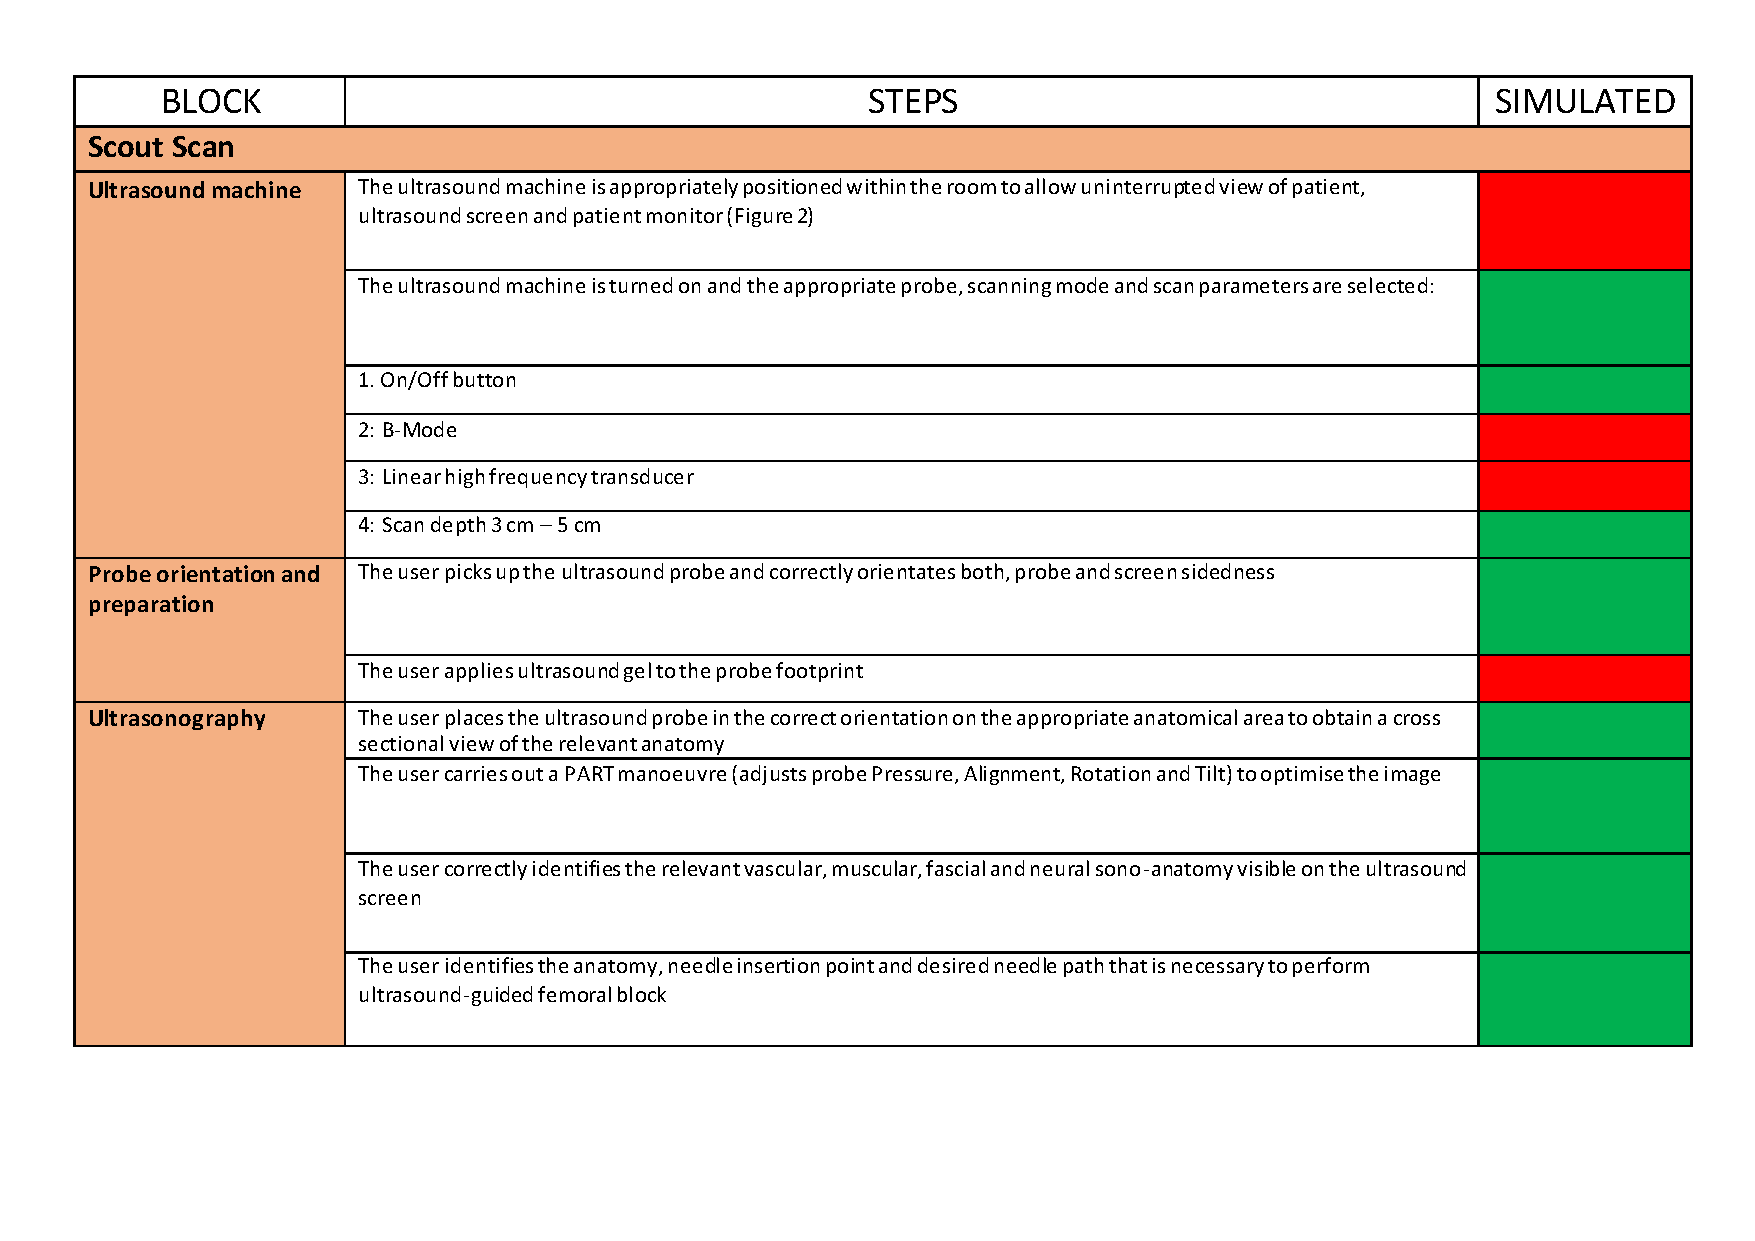
\includepdf[pages=1,frame,landscape]{PDFs/RA} 
% \includepdf[pages=2,frame,landscape]{PDFs/RA}
% \includepdf[pages=3,frame,landscape]{PDFs/RA}
\begin{figure}[ht]
    \centering
    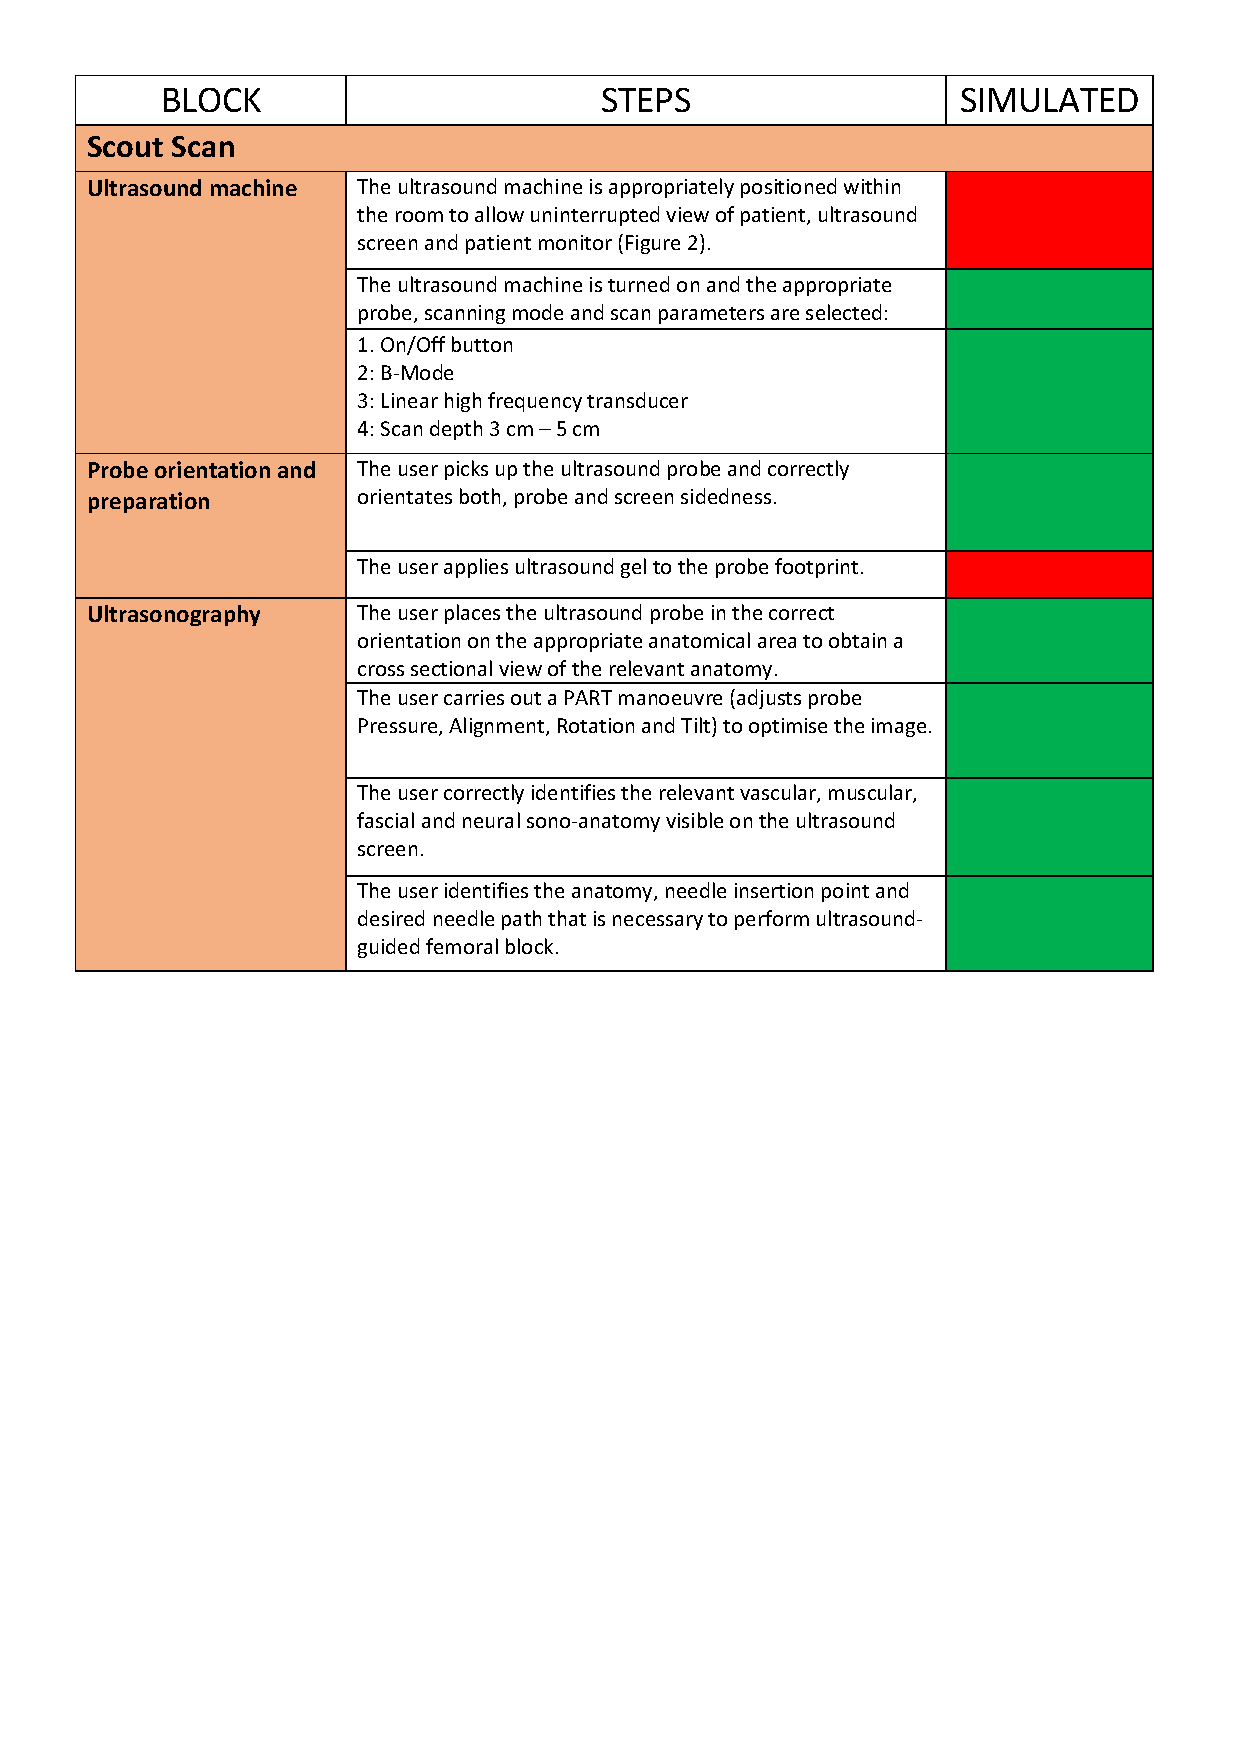
\includegraphics[trim={1cm 13cm 1cm 1cm},clip,width=0.9\textwidth]{PDFs/RA1.pdf}
       \caption{Relación entre las etapas de la exploración del procedimiento de \acs{RA} y si la funcionalidad del simulador \acs{RASim} está simulada.\label{fig:RAsteps1} }
    
\end{figure}
\begin{figure}[ht]
    \centering
    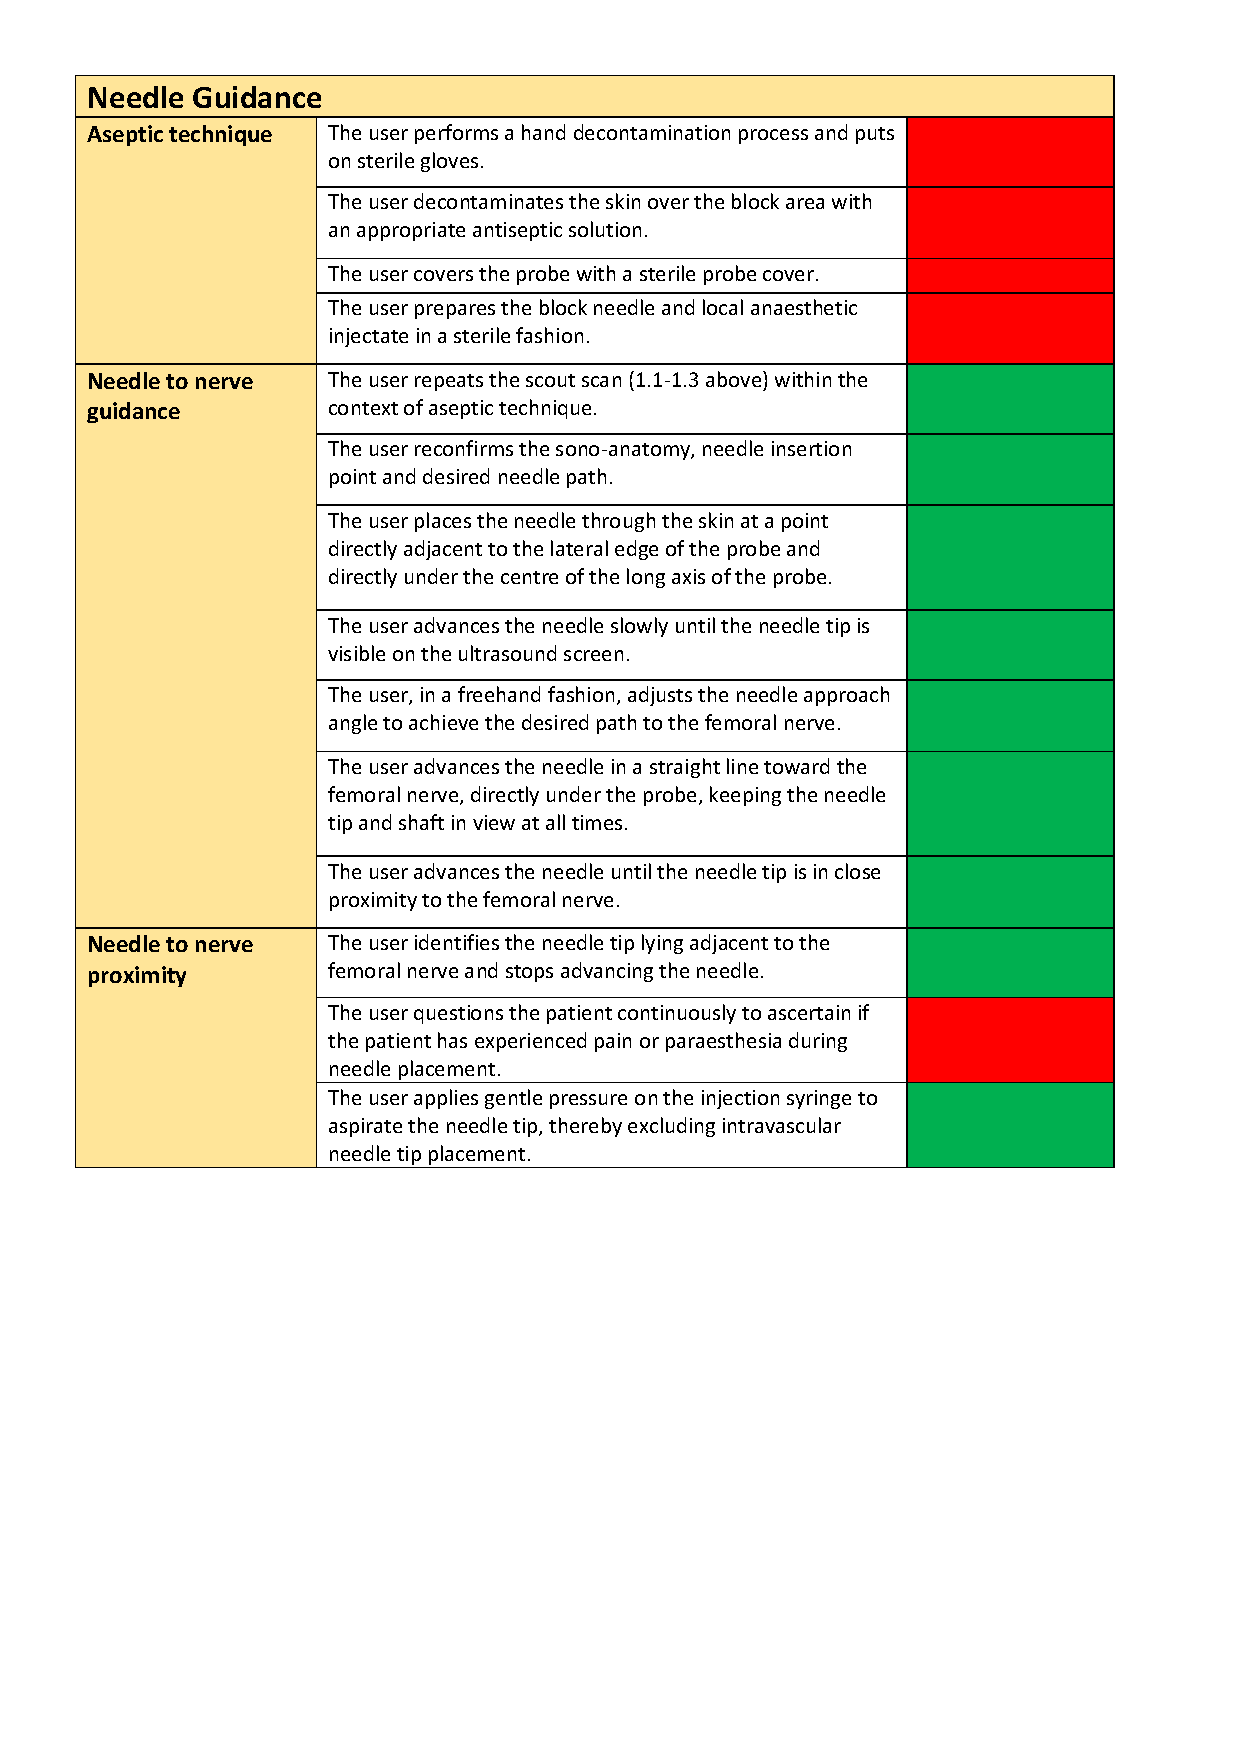
\includegraphics[trim={1cm 85mm 1cm 1cm},clip,width=0.9\textwidth]{PDFs/RA2.pdf}
       \caption{Relación entre las etapas de la fase de guiado de la aguja del procedimiento de \acs{RA} y si la funcionalidad del simulador \acs{RASim} está simulada.\label{fig:RAsteps2} }
    
\end{figure}
\begin{figure}[ht]
    \centering
    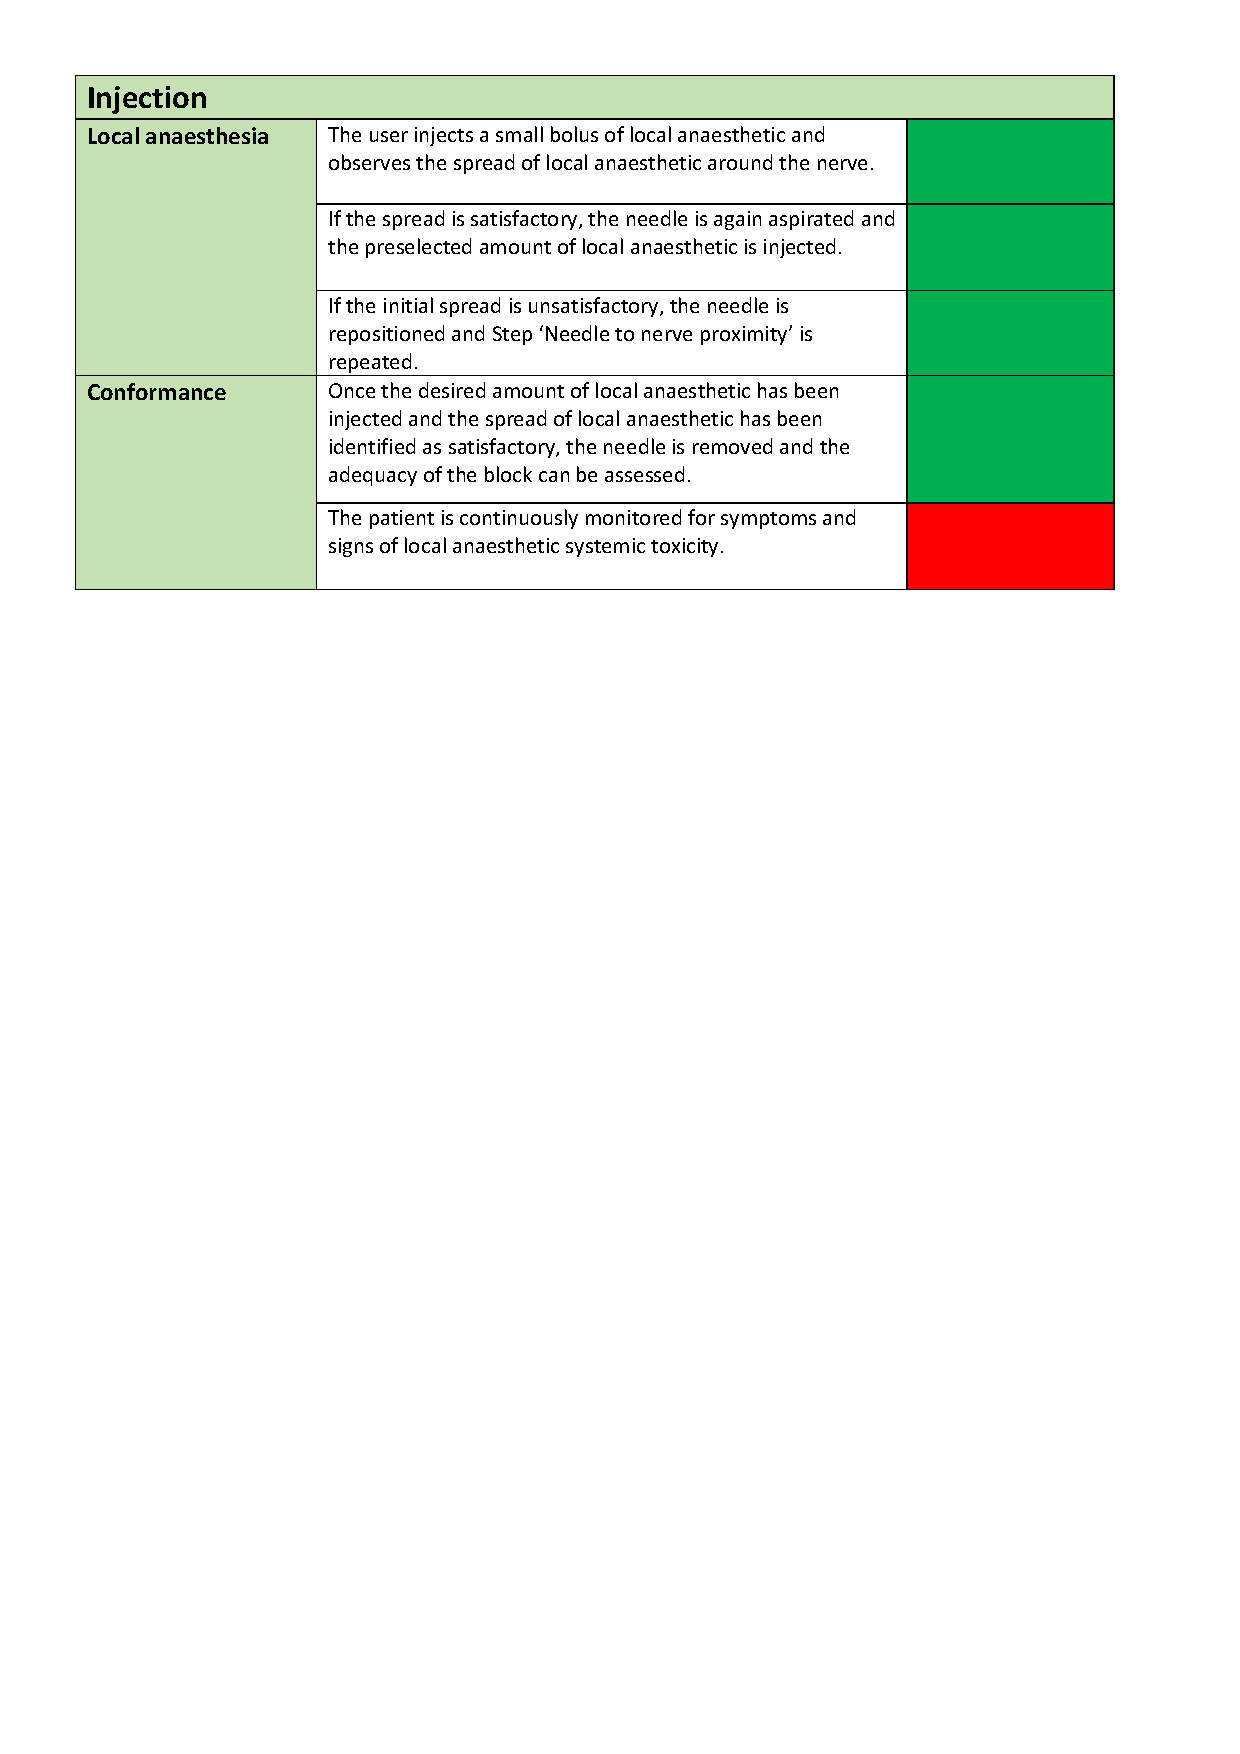
\includegraphics[trim={1cm 19cm 1cm 1cm},clip,width=0.9\textwidth]{PDFs/RA3.pdf}
       \caption{Relación entre las etapas de la fase de inyección del procedimiento de \acs{RA} y si la funcionalidad del simulador \acs{RASim} está simulada.\label{fig:RAsteps3} }
    
\end{figure}



Además de la caracterización correcta de las distintas fases del procedimiento, el \ac{Courseware} permite la ejecución del modo guiado y modo libre. Los médicos evaluaron de forma positiva la introducción de un modo guiado que ayude y permita mejorar la seguridad del estudiante antes de realizar el modo libre sin ninguna experiencia previa. Este modo guiado permite suministrar retroalimentación formativa para mejorar el aprendizaje del usuario. Por otra parte, al final de la sesión ambos modos muestran al usuario una ventana de resultados donde se proporciona una retroalimentación sumativa. Esto es posible gracias a la recolección de métricas por parte del simulador. Junto con los médicos del proyecto se especificaron aquellas que debían ser registradas por el simulador para poder realizar una evaluación del estudiante. En el documento \cite{ded4.4}, se pueden consultar de manera pormenorizadas.

%Por otra parte, se negoció las métricas que el simulador debería recoger para evaluar correctamente tanto formativa como sumativa.



%\subsection{Rendimiento}
%%%%%
% En algún lado (ya no se donde) deberías haber contado que hubo problemas con el phantom omni. (Si esta en conclusiones muévelo aquí. si esta antes esta bien.) Cuando muevas cosas, asegúrate que las sección fuente y destino son coherentes. 
% 1. Se requeria retroalimentación haptica para localizar la aguja
%2. bajo precio
% 3.  Se opta por el OMNI
%4. La nuevea version tiene problemas
%5. Los medicos no permite su paso a fase de esayo clinico.
%6. Tu desarrollas una solucion basda en el tracker. 
%7. El equipo de Cork no da validación conceptual:
%8. US, Deformación 
%9. Courware. Aquí dedica más tiempo. Di que fases etapas se pueden entrenar y cuales no. 
%10. Deja claro que no se puede ni liberar el anestesico, ni confirar que el bloqueo es positivo, pero el resto se puede hacer. 

En relación al prototipo completo, en términos computacionales, el sistema es capaz de satisfacer los requisitos de interactividad que se le presuponen a un simulador de \ac{RV}. El simulador \ac{RASim} muestra una ejecución interactiva en todas las etapas incluyendo aquellas computacionalmente más costosas. Por ejemplo, el sistema es capaz de responder con fluidez cuando el usuario introduce la aguja y se devuelve retroalimentación háptica, a la vez que se sigue ejecutando la simulación de la imagen de \ac{US}. El usuario no percibía en ningún caso un retraso de las respuestas físicas o de las imágenes mostradas por los monitores.

Con el objetivo de verificar que las habilidades adquiridas con el simulador se pueden transferir a situaciones reales, se deben realizar validaciones de constructo, concurrente y predictiva. Estaba previsto realizarse en un ensayo clínico pero, lamentablemente, la validación del simulador completo no ha sido posible por diversas dificultades.

Cuando se disponía a realizar la evaluación de apariencia del prototipo antes del ensayo clínico, se descubrió que los prototipos habían sufrido daños en el transcurso de su transporte. % Los principales componentes del computador habían quedado inservibles, en concreto la \ac{GPU}. Estos desperfectos dieron lugar a replantear la planificación de las evaluaciones del prototipo.
En cuanto se pudo resolver este problema, se procedió a presentar los dispositivos al comité médico para comprobar y realizar una validación aparente. Por su parte, los médicos expresaron ciertas preocupaciones sobre la falta de correspondencia entre la posición del dispositivo y su representación virtual. Debido a la falta de equivalencia entre la posición de la aguja y la sonda de \ac{US}, no era posible que el usuario obtuviera una imagen clara de la aguja en el procedimiento, y esto podría ocasionar malas prácticas y sesgos en los aprendices. 

En la figura \ref{fig:errorhaptic}, se puede apreciar que la rotación del actuador del dispositivo \emph{Touch}  no correspondía con los valores recogidos por el software de calibración. Para ilustrar la desviación que sufrían, se rotaba el dispositivo hasta el punto en el que marcaba una rotación simple de $90$ grados, pero el actuador se encontraba más allá de la horizontal. Además, se comprobó que por cada dispositivo el error era diferente. Se determinó y confirmó con el fabricante que los dispositivos sufrían de un defecto de hardware de fábrica. Se puede revisar con más detalle el informe que se envió al fabricante en el anexo \ref{anexo:geomagic}.


\begin{figure}[ht]
\centering
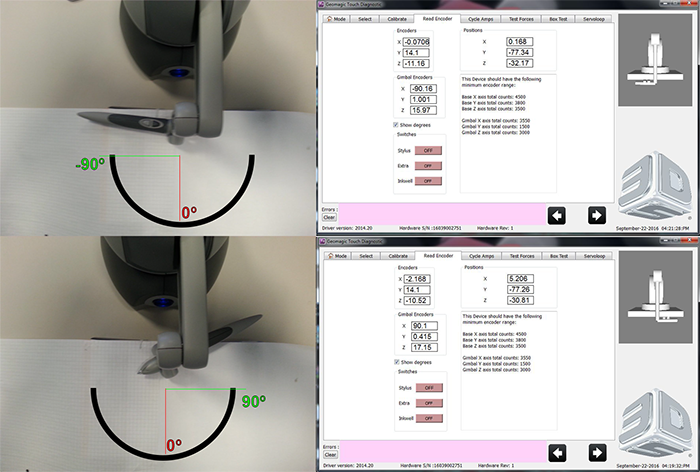
\includegraphics[width=0.9\linewidth]{IMG/errorhaptic.png}
\caption{\label{fig:errorhaptic}Diferencias de rotaciones reales frente a las proporcionadas por el dispositivo a través de su herramienta de calibración.}
\end{figure}

%Con la esperanza de una solución, se contactó con la empresa que ha distribuido los dispositivos. La empresa detectó este mismo error en los dispositivos de nueva facturación y comunicó que propondrían una solución para ello. Esta solución no ha llegado en un tiempo razonable en la que permitiera proceder a la evaluación del prototipo en un entorno clínico. A su vez, 
%Se propusieron alternativas para los dispositivos, como por ejemplo utilizar solo \ac{tracker}s sacrificando la respuesta háptica. 


A partir de una propuesta de la \ac{URJC}, se sustituyeron los dispositivos hápticos por unos \emph{\acs{tracker}s} magnéticos que permitieron conseguir una evaluación favorable del prototipo para proceder a su evaluación  en un entorno clínico. Debido a la conclusión del proyecto y, por tanto, a la falta de recursos económicos, no se ha podido realizar el ensayo clínico.



%Aunque, debido a estos problemas, no se ha re evaluación clínica antes de la finalización del proyecto.
%\todo{Marcos says:da  validez aparente al prototipo de RASim con trackers}
%4clínica oportunas entre las que se propusieron: validez predictiva, de contenido y de constructo.





% \subsection{Discusión}
% \label{rasim:discusion}

%\ac{RASim} presenta una carencia fundamental  carencias frente al procedimiento de \ac{RA}. 
% Como ha sido comentado anteriormente, el simulador \ac{RASim} presenta problemas con el dispositivo háptico. La respuesta física del movimiento de la aguja es un punto fundamental en el entrenamiento del procedimiento. Aunque este módulo ha sido validado correctamente fuera del simulador \cite{needleinsertion}, no ha sido posible su correcta validación en el prototipo \ac{RASim}.
%Por otra parte, en cuanto a la imagen de \ac{US}, la principal queja a la que se enfrenta el simulador es que proporciona una imagen, aunque parecida, demasiado clara y perfecta y no refleja completamente las dificultades que se presentan las imágenes ultrasónicas reales.

% En primer lugar, es importante comentar el resultado final de la evaluación de la comisión europea sobre el proyecto \ac{RASimAs}. Este comité califico el proyecto con un \emph{progreso aceptable} debido a las dificultades para finalizar la evaluación clínica. Los problemas inesperados fueron los determinantes para que esta evaluación no pudiera hacerse en el tiempo esperado. Aun así, se valoró muy positivamente el módulo de \ac{RAAs} y el estado del prototipo final de \ac{RASim}. El propio comité animó a seguir con los trabajos necesarios que hagan falta para la finalización del \ac{RASim} y que pueda ser utilizado en entornos reales para el beneficio de los estudiantes de anestesiología.

%Este fallo no se había producido en el desarrollo del prototipo y no estaba presente en los equipos de desarrollo. 

%Entre los participantes del desarrollo del prototipo se descubrió que los errores de precisión provenían de los dispositivos hápticos. Estos no proporcionaban una rotación adecuada según su posición real como se puede observar en la figura \ref{fig:errorhaptic}.
% En las imágenes, se puede apreciar que la rotación del actuador no corresponde con los valores recogidos por el software, por lo tanto, no habría una correspondencia directa. Para ilustrar la desviación que causaban, se rotaba el dispositivo hasta el punto en el que marcaba una rotación simple de 90 grados, pero el actuador se encontraba más allá de la horizontal. Además, por cada dispositivo, el error era diferente, por lo cual no cabía la posibilidad de crear una solución única para todos los prototipos. También se podía inducir que el problema parecía ser de \emph{hardware} y no un error del \emph{software} del dispositivo.


% \begin{figure}[ht]
% \centering
% 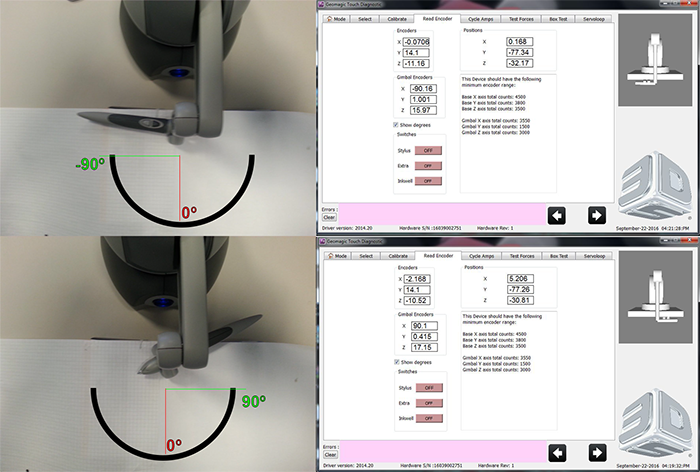
\includegraphics[width=0.9\linewidth]{IMG/errorhaptic.png}
% \caption{\label{fig:errorhaptic}Diferencias de rotaciones reales frente a las proporcionadas por el dispositivo a través de su herramienta de calibración.}
% \end{figure}

%Con la esperanza de una solución, se contactó con la empresa que ha distribuido los dispositivos. La empresa detectó este mismo error en los dispositivos de nueva facturación y comunicó que propondrían una solución para ello. Esta solución no ha llegado en un tiempo razonable en la que permitiera proceder a la evaluación del prototipo en un entorno clínico. A su vez, 
%Se propusieron alternativas para los dispositivos, como por ejemplo utilizar solo \ac{tracker}s sacrificando la retroalimentación háptica, la cual era un punto fundamental del proyecto. Debido a la conclusión del proyecto y, por tanto, la falta de recursos económicos no se ha podido completar ninguna alternativa en el tiempo necesario para realizar una validación en un entorno clínico.



%Por último, hay que tener en cuenta que ciertos aspectos protocolarios del procedimiento no están incluidos en el simulador, como tampoco se encuentra la simulación de las tareas de la técnica aséptica.




